\documentclass{article}
\usepackage{amsmath,amssymb,graphicx,tikz}

\begin{document}
\setlength{\parindent}{0pt}


% \begin{center}
%     {\LARGE \textbf{Problem set 2}}
% \end{center}
% \vspace{0.5cm}


% \textbf{1.\ (Binary stones).}
Consider the following game: two players may take from a heap any number of stones that is a power of \(2\) (including \(1 = 2^0\)).
The player who has taken the last stone wins.
For which number of stones does the first player win?
How should he play?
(You should not only specify the strategy but also prove that it works.)

\textbf{Solution.}

Let \(n\) be the number of stones.
Allowed moves are to remove \(1, 2, 4, 8, \dots, 2^k\) stones.
We seek the losing positions:

\medskip
\noindent\textbf{Small cases.}
\[
\begin{array}{c|cccccccccc}
n & 0 & 1 & 2 & 3 & 4 & 5 & 6 & 7 & 8 & 9\\\hline
\text{outcome} & \text{lose} & \text{win} & \text{win} & \text{lose} & \text{win} & \text{win} & \text{lose} & \text{win} & \text{win} & \text{lose}
\end{array}
\]
The losing positions among these are \(0, 3, 6, 9, \dots\)

\medskip
\noindent\textbf{Claim.}
The losing positions are exactly the multiples of \(3\).
Equivalently, the first player wins if and only if \(n \not\equiv 0 \pmod{3}\). For example, 1, 2 or 4 and etc.

\medskip
\noindent\textbf{Proof.}
Powers of \(2\) modulo \(3\) alternate:
\[
2^0 \equiv 1\pmod{3} \qquad 2^1 \equiv 2\pmod{3}
\]
\[
2^2 \equiv 1 \pmod{3} \qquad 2^3 \equiv 2 \pmod{3}
\]
In general \(2^k \equiv (-1)^k \pmod{3}\), so every allowed move removes either \(1\) or \(2\) modulo \(3\), never \(0\) modulo \(3\).

\smallskip
If \(n \equiv 0 \pmod{3}\), then for any move \(n \mapsto n - 2^k\) we have \(n - 2^k \not\equiv 0 \pmod{3}\).

If \(n \not\equiv 0 \pmod{3}\), there is a move to a multiple of \(3\):

\begin{center}

\noindent\textbf{1.} \(n \equiv 1 \pmod{3}\), remove \(1 = 2^0\)

\noindent\textbf{2.} \(n \equiv 2 \pmod{3}\), remove \(2 = 2^1\)

\end{center}

Thus from a multiple of \(3\) every move goes to a non-multiple of \(3\), and from a non-multiple of \(3\) there is a move to a multiple of \(3\).
The terminal position \(n = 0\) is a multiple of \(3\) and is losing for the player to move.
Hence multiples of \(3\). Therefore the first player wins if and only if \(n \not\equiv 0 \pmod{3}\).

\medskip
\noindent\textbf{Optimal strategy.}
If \(n \equiv 1 \pmod{3}\), remove \(1\) stone; if \(n \equiv 2 \pmod{3}\), remove \(2\) stones.
Thereafter always leave a heap size divisible by \(3\).
Since the opponent can only subtract \(1\) or \(2\) modulo \(3\) from the heap, you can always restore divisibility by \(3\) on your turn.
Eventually the opponent faces \(n = 0\) and loses.

% \vspace{1cm}

% \textbf{2.\ (Moving the knight).}

We number the board by coordinates
\[
a1=(1,1),\qquad h8=(8,8).
\]
The knight starts at
\[
h8=(8,8).
\]

A legal move is one of
\[
(x,y)\mapsto (x+1,y-2),
\]
\[
(x,y)\mapsto (x-1,y-2),
\]
\[
(x,y)\mapsto (x-2,y+1),
\]
\[
(x,y)\mapsto (x-2,y-1)
\]
provided the new square is still on the board.
winning if the player to move from it can move to a losing position.

\subsection*{Losing positions on the \(8\times 8\) board}

In coordinates, these are the \(2\times2\) blocks
\[
\{1,2\}\times\{1,2\},
\]
\[
\{1,2\}\times\{5,6\},
\]
\[
\{5,6\}\times\{1,2\},
\]
\[
\{5,6\}\times\{5,6\},
\]
together with the special square
\[
(8,8).
\]

We can see that losing positions satisfy
\[
x,y\equiv 1 \text{ or } 2 \pmod 4
\]

On the \(8\times 8\) board, the losing positions can be displayed as follows:

\[
\begin{array}{c|cccccccc}
& 1 & 2 & 3 & 4 & 5 & 6 & 7 & 8\\
\hline
8 & . & . & . & . & . & . & . & L\\
7 & . & . & . & . & . & . & . & .\\
6 & L & L & . & . & L & L & . & .\\
5 & L & L & . & . & L & L & . & .\\
4 & . & . & . & . & . & . & . & .\\
3 & . & . & . & . & . & . & . & .\\
2 & L & L & . & . & L & L & . & .\\
1 & L & L & . & . & L & L & . & .
\end{array}
\]

\subsection*{Why these positions are losing}

Let
\[
R=\{(x,y): x,y\equiv 1 \text{ or }2 \pmod 4\}.
\]

These positions form repeated \(2\times2\) blocks. A knight move changes one
coordinate by \(1\) and the other coordinate by \(2\). Therefore a move from a
position in \(R\) always leaves \(R\). So no position in \(R\) has a move to
another position in \(R\).

Conversely, by backward induction, every legal move out of one of these blocks
leads to a position from which the next player can move back into a smaller
\(R\)-position. Hence the positions in \(R\) are losing.

Now check the starting square:
\[
h8=(8,8)
\]
Its only legal moves are
\[
(8,8)\mapsto (7,6)
\]
and
\[
(8,8)\mapsto (6,7)
\]

Both of these positions are winning, because both can move to
\[
(5,5)=e5,
\]
which is losing:
\[
(7,6)\mapsto (5,5),
\]
\[
(6,7)\mapsto (5,5)
\]

Therefore every legal move from \(h8\) goes to a winning position. Hence
\[
h8
\]
is losing.

Thus the first player loses and the second player wins.

% \subsection*{General \(n\times n\) board}

% For the same game on an \(n\times n\) board, the losing block pattern repeats
% modulo \(4\): positions with
% \[
% x,y\equiv 1 \text{ or }2 \pmod 4
% \]
% are losing.

% Starting from \((n,n)\), if \(n\equiv1\) or \(2\pmod4\), the initial square is
% already losing. If \(n\equiv3\pmod4\), the first player moves
% \[
% (n,n)\mapsto(n-1,n-2),
% \]
% which has residue \((2,1)\) and is losing. If \(n\equiv0\pmod4\), the only
% first moves go to \((n-1,n-2)\) or \((n-2,n-1)\), and each can be answered by
% moving to \((n-3,n-3)\equiv(1,1)\pmod4\), a losing square.

% Thus, on an \(n\times n\) board starting from the top-right corner,

% \[
% \boxed{\text{the first player wins if and only if } n\equiv 3\pmod4.}
% \]

% For the usual chessboard,
% \[
% 8\equiv0\pmod4,
% \]
% so the first player loses and the second player wins.

\section*{Moving the knight: general solution}

Consider an \(n\times n\) board with coordinates
\[
(1,1), (1,2), \ldots, (n,n),
\]
where the knight starts at the top-right corner
\[
(n,n).
\]

The legal moves are the same as before whenever the new square is still on the board.


\subsection*{Losing blocks}

The basic losing positions are the \(2\times2\) blocks satisfying
\[
x,y\equiv 1 \text{ or } 2 \pmod 4.
\]


A move from such a square always leaves this set. Moreover, after any legal move from such a square, the next player can move back to a smaller square of the same type. Therefore these positions are losing positions.

\subsection*{Starting from the corner}

Now consider the starting square
\[
(n,n).
\]

There are four cases.

\subsubsection*{Case 1: \(n\equiv1\pmod4\)}

Then
\[
(n,n)\equiv(1,1)\pmod4,
\]
so \((n,n)\) lies in a losing block. Hence the first player loses.

\subsubsection*{Case 2: \(n\equiv2\pmod4\)}

Then
\[
(n,n)\equiv(2,2)\pmod4,
\]
so \((n,n)\) also lies in a losing block. Hence the first player loses.

\subsubsection*{Case 3: \(n\equiv3\pmod4\)}

Then the first player can move
\[
(n,n)\mapsto(n-1,n-2)
\]
Modulo \(4\), this is
\[
(3,3)\mapsto(2,1)
\]
Since \((2,1)\) is a losing-type residue, the first player can move to a losing position. Hence the first player wins.

\subsubsection*{Case 4: \(n\equiv0\pmod4\)}

The square \((n,n)\) is not itself in the losing block pattern. However, because it is the top-right corner, it has only two legal moves:
\[
(n,n)\mapsto(n-1,n-2),
\]
\[
(n,n)\mapsto(n-2,n-1)
\]

Both resulting positions are winning, because from either one the next player can move to
\[
(n-3,n-3).
\]

Indeed,
\[
(n-1,n-2)\mapsto(n-3,n-3),
\]
and
\[
(n-2,n-1)\mapsto(n-3,n-3)
\]

Since
\[
n\equiv0\pmod4,
\]
we have
\[
n-3\equiv1\pmod4
\]
Therefore
\[
(n-3,n-3)\equiv(1,1)\pmod4,
\]
which is a losing block position.

Thus every legal move from \((n,n)\) gives the opponent a move to a losing position. Hence \((n,n)\) is losing.

\subsection*{Conclusion}

Therefore, on an \(n\times n\) board starting from the top-right corner,
\[
\text{the first player wins if and only if } n\equiv3\pmod4
\]

For the usual chessboard,
\[
8\equiv0\pmod4,
\]
so the first player loses and the second player wins.

% \vspace{1cm}

% \textbf{3.\ (Pawn duel).}
Consider the following game on a \(3\times 8\) table.
Each of the two players has three pawns along the short edges.
During the first turn each player may move any of his pawns towards the opposite
edge but not further than by \(3\) cells.
During the later rounds each player may move any of his pawns towards the
opposite edge by any number of cells.
The players cannot move the pawns vertically or diagonally, nor can they jump
across or take pawns of the other player.
The player that has no legal turn loses.
Which player has a winning strategy?
How should he play?

\textbf{Solution.}

For each of the three rows, let
\[
d_i=\text{the number of empty cells between the two pawns in row } i
\]

Initially, in each row the two pawns stand at opposite ends of an \(8\)-cell row, so
\[
d_1=d_2=d_3=6
\]
Thus the initial position is
\[
(6,6,6)
\]

A move in one row simply decreases exactly one of the numbers \(d_i\) by a positive amount. Hence, after the first restricted moves, the game is equivalent to Nim with three heaps of sizes
\[
d_1,d_2,d_3
\]

In Nim, a position is losing if and only if
\[
d_1\oplus d_2\oplus d_3=0,
\]
where \(\oplus\) denotes bitwise XOR.

The initial Nim-sum is
\[
6\oplus 6\oplus 6 = 6\neq 0
\]
Indeed, in binary this is
\[
110_2\oplus 110_2\oplus 110_2 = 110_2
\]

The first player should move one pawn forward by exactly \(2\) cells. This changes one gap from \(6\) to \(4\), so the position becomes
\[
(4,6,6).
\]

Now
\[
4\oplus 6\oplus 6 = 4
\]

If the second player wanted to make the Nim sum zero immediately, he would have to change one heap \(h\) into
\[
h' = h\oplus 4
\]

The possible changes for \(h\) are :

\(h=4\):
\[
4\to 4\oplus 4 = 0,
\]
or for \(h=6\):
\[
6\to 6\oplus 4 = 2
\]

Both moves require decreasing a gap by \(4\). But on the second player's first move, he is allowed to move a pawn by at most \(3\) cells. Therefore, the second player cannot move to a zero Nim-sum position.

After that, the first player is no longer restricted. From then on he uses the standard Nim strategy: after every move of the opponent, make
\[
d_1\oplus d_2\oplus d_3=0
\]

For example, after the first move
\[
(6,6,6)\to(4,6,6),
\]
the second player's first move can produce, up to permutation of rows, only one of the following positions:
\[
(3,6,6),\quad (2,6,6),\quad (1,6,6),
\]
or
\[
(4,5,6),\quad (4,4,6),\quad (4,3,6)
\]

The first player answers as follows:
\[
(3,6,6)\to(0,6,6),
\]
\[
(2,6,6)\to(0,6,6),
\]
\[
(1,6,6)\to(0,6,6),
\]
\[
(4,5,6)\to(3,5,6),
\]
\[
(4,4,6)\to(4,4,0),
\]
\[
(4,3,6)\to(4,2,6)
\]

In each case the resulting Nim-sum is zero.

Thus the first player can always give the second player a position satisfying
\[
d_1\oplus d_2\oplus d_3=0.
\]

The game eventually ends.
Since the first player always leaves the second player a zero Nim sum position, the second player is the one who eventually has no legal move.

\smallbreak
Therefore, the first player has a winning strategy.

\[
\text{The first player wins.}
\]

His strategy is:

\[
\text{First move: move any pawn forward by exactly }2\text{ cells.}
\]

After that, always move so that
\[
d_1\oplus d_2\oplus d_3=0
\]

% \vspace{1cm}

% \textbf{4.\ (Cake division).}

Albert and Bernie divide a cake by alternating proposals. First Albert proposes
a division. If Bernie accepts, the division is implemented. Otherwise they wait
one hour and Bernie proposes. If Albert accepts, the division is implemented;
otherwise they wait another hour, and so on.

A fraction \(p\) of the cake is worth
\[
p\left(\frac12\right)^t
\]
after \(t\) hours of waiting, for \(t\le 5\). After \(5\) hours the cake becomes
worthless. Find a subgame perfect Nash equilibrium and determine how long they wait.

\textbf{Solution.}

The last possible valuable proposal is at \(t=5\), made by Bernie. If Albert
rejects at \(t=5\), both get \(0\). Hence Bernie can keep the whole remaining cake:
\[
V_5^P=\left(\frac12\right)^5=\frac1{32}
\]

Applying backward induction. At time \(t\), the responder can reject and become proposer at
time \(t+1\). Therefore the responder must receive exactly the value with which the responder would accept the proposal
\[
V_{t+1}^P -
\]

Hence
\[
V_t^P=\left(\frac1{2}\right)^t - V_{t+1}^P
\]

Now compute with \(V_6=0\):
\[
V_5^P=\left(\frac1{2}\right)^5 - V_6=\frac1{32} - 0=\frac1{32},
\]
\[
V_4^P=\left(\frac1{2}\right)^4 - V_5=\frac1{16} - \frac1{32}=\frac1{32},
\]
\[
V_3^P=\left(\frac1{2}\right)^3 - V_4=\frac1{8} - \frac1{16}=\frac3{32},
\]
\[
V_2^P=\left(\frac1{2}\right)^2 - V_3=\frac1{4} - \frac3{32}=\frac5{32},
\]
\[
V_1^P=\left(\frac1{2}\right)^1 - V_2=\frac1{2} - \frac5{32}=\frac{11}{32},
\]
\[
V_0^P=\left(\frac1{2}\right)^0 - V_1=\frac{21}{32}
\]

At \(t=0\), Albert is proposer. He gives Bernie her continuation value:
\[
\frac{11}{32}
\]

Therefore Albert proposes
\[
\left(\frac{21}{32},\frac{11}{32}\right),
\]
and Bernie accepts.

Thus the subgame perfect Nash equilibrium outcome is
\[
\left(\frac{21}{32},\frac{11}{32}\right)
\]
and they wait
\[
0\text{ hours}
\]

% \vspace{1cm}

% \textbf{5.\ (Pirates and treasure).}
50 pirates ordered by rank are dividing a big treasure that consists of 1000
equal indivisible items. They employ the following procedure. Firstly, the
captain offers a division. If at least half of the crew (including the captain)
agree, then the division is applied. Otherwise the captain is thrown overboard
and the second-ranked pirate offers a division, and so on. Formalize the
situation as a dynamic game and find a subgame perfect Nash equilibrium such
that no pirate is indifferent at any time.

\textbf{Solution.}

Consider a subgame with \(n\) surviving pirates, relabeled
\[
1,2,\dots,n,
\]
where pirate \(1\) is the proposer. A proposal passes if it gets at least
\[
\left\lceil \frac n2 \right\rceil
\]
votes. Since the proposer votes for himself, he needs
\[
\left\lceil \frac n2 \right\rceil -1
=
\left\lfloor \frac{n-1}{2}\right\rfloor
\]
additional votes.

Using backward induction. A pirate votes yes only if he gets strictly more than
he would get after rejecting the proposal. We also don't want to pay the next possible captain and we pay only to those pirates
who would get 0 if a proposal is rejected.

% For small \(n\), the pattern is:
% \[
% n=1:\quad (1000),
% \]
% \[
% n=2:\quad (1000,0),
% \]
% \[
% n=3:\quad (999,1,0),
% \]
% \[
% n=4:\quad (999,1,0,0),
% \]
% \[
% n=5:\quad (998,1,1,0,0)
% \]

For small \(n\), the pattern is:
\[
n=1:\quad (1000),
\]
\[
n=2:\quad (1000,0),
\]
\[
n=3:\quad (999,0,1),
\]
\[
n=4:\quad (999,0,1,0),
\]
\[
n=5:\quad (998,0,1,0,1)
\]


Thus, in a subgame with \(n\) pirates, the proposer buys the cheapest votes:
pirates
\[
3,5,7,\dots
\]
each get \(1\) item, and the others get \(0\).

For \(n=50\), the captain needs
\[
\left\lceil \frac{50}{2}\right\rceil =25
\]
votes total. His own vote counts, so he needs \(24\) more votes.

He gives \(1\) item to pirates
\[
3,5,7,\dots,49.
\]

There are \(24\) such pirates. Therefore the captain keeps
\[
1000-24=976.
\]

Hence the equilibrium proposal is
\[
(x_1,x_2,\dots,x_{50})
=
(976,0,1,0,1,0,\dots,1,0)
\]
where
\[
x_1=976,
\]
\[
x_{3}=x_{5}=\cdots=x_{49}=1,
\]
and
\[
x_2=x_4=\cdots=x_{50}=0
\]

The yes-voters are
\[
\{1,3,5,\dots,49\},
\]
which gives exactly \(25\) votes, so the proposal passes.

Therefore, in the subgame perfect Nash equilibrium, the first captain survives
and keeps
\[
976
\]
items.

% \vspace{1cm}

% \textbf{6.\ (Dormitory shopping).}
Anna and Belle live in the same dormitory. They go shopping every day, and
shopping takes \(20\) minutes. They decided to cooperate for \(4\) days:
on Monday Anna buys food for both of them, on Tuesday Belle does the same,
on Wednesday Anna again, and on Thursday Belle again.

Buying food for the mate takes \(5\) extra minutes. Thus, the assigned shopper
has an incentive to break the rule. If any agent does not buy food for the mate,
then both go shopping by themselves for the rest of the game.

Formalize the situation as a dynamic game and find all subgame perfect Nash
equilibria.

\textbf{Solution.}

Let
\[
c=\text{``buy for both''},\qquad d=\text{``buy only for yourself''}
\]

If someone chooses \(d\), cooperation ends and both shop separately for the rest
of the game. Payoffs are negative total shopping time.

Use backward induction.

On Thursday, Belle chooses between
\[
c:25,\qquad d:20
\]
Thus Belle chooses \(d\).

On Wednesday, Anna knows Belle will defect on Thursday. If Anna cooperates, her
remaining cost is
\[
25+20=45
\]
If Anna defects, her remaining cost is
\[
20+20=40
\]
Thus Anna chooses \(d\).

On Tuesday, Belle knows Anna will defect on Wednesday. If Belle cooperates, her
remaining cost is
\[
25+20+20=65.
\]
If Belle defects, her remaining cost is
\[
20+20+20=60.
\]
Thus Belle chooses \(d\).

On Monday, Anna knows Belle will defect on Tuesday. If Anna cooperates, her
total cost is
\[
25+20+20+20=85.
\]
If Anna defects, her total cost is
\[
20+20+20+20=80.
\]
Thus Anna chooses \(d\).

Therefore the unique subgame perfect Nash equilibrium is
\[
s_A=(d,d),\qquad s_B=(d,d)
\]

That is, each player defects whenever it is her turn to buy.

On the equilibrium path, Anna defects immediately on Monday. Then both shop
alone every day. Hence total shopping times are
\[
(80,80)
\]

The agreement is therefore not subgame perfect.

% \vspace{1cm}

% \newpage


\begin{center}
    {\LARGE \textbf{Problem set 3}}
\end{center}
\vspace{0.5cm}

\textbf{1.\ (Filming a movie).}
A producer (Polly), an operator (Oliver) and a composer (Chris) are filming a
movie. The movie yields \(\$10000\) profit. Oliver himself can earn \(\$2000\)
by filming a wedding, Chris himself can earn \(\$3000\) by selling the music,
Polly herself can earn only \(\$1000\) by event management. Oliver and Chris
can earn \(\$6000\) by creating a music film for a wedding. Oliver and Polly
can earn \(\$4000\) by organizing the whole wedding. Polly and Chris can earn
\(\$4500\) by organizing a party.

\begin{enumerate}
    \item[(a)] Formalize the situation as a coalitional game. Is it superadditive?
    Supermodular?
    \item[(b)] Find the core and draw it on the plane (Polly payoff, Chris payoff).
    \item[(c)] Find the Shapley value. Does it lie inside the core?
\end{enumerate}

\textbf{Solution.}

Let
\[
N=\{P,O,C\},
\]
where \(P\) is Polly, \(O\) is Oliver, and \(C\) is Chris.

The payoff function is
\[
v(\varnothing)=0,
\]
\[
v(P)=1000,\qquad v(O)=2000,\qquad v(C)=3000,
\]
\[
v(PO)=4000,\qquad v(PC)=4500,\qquad v(OC)=6000,
\]
\[
v(POC)=10000
\]

The game is superadditive, since every coalition gives at least as much
as separate coalitions. Showing this:

\[
v(PO)=4000\ge v(P)+v(O)=1000+2000=3000,
\]
\[
v(PC)=4500\ge v(P)+v(C)=1000+3000=4000,
\]
\[
v(OC)=6000\ge v(O)+v(C)=2000+3000=5000,
\]
\[
v(POC)=10000\ge v(P)+v(OC)=1000+6000=7000,
\]
\[
v(POC)=10000\ge v(O)+v(PC)=2000+4500=6500,
\]
\[
v(POC)=10000\ge v(C)+v(PO)=3000+4000=7000
\]


Hence the game is superadditive.


Show supermodularity:
\[
v(POC)+v(P)\ge v(PO)+v(PC),
\]
because
\[
10000+1000=11000\ge 4000+4500=8500
\]
Similarly,
\[
v(POC)+v(O)\ge v(PO)+v(OC),
\]
because
\[
10000+2000=12000\ge 4000+6000=10000
\]
And
\[
v(POC)+v(C)\ge v(PC)+v(OC),
\]
because
\[
10000+3000=13000\ge 4500+6000=10500
\]
So, the game is supermodular.


\medskip
The core consists of allocations
\[
x=(x_P,x_O,x_C)
\]
such that
\[
x_P+x_O+x_C=10000,
\]
and
\[
x_P\ge1000,\qquad x_O\ge2000,\qquad x_C\ge3000,
\]
\[
x_P+x_O\ge4000,
\]
\[
x_P+x_C\ge4500,
\]
\[
x_O+x_C\ge6000
\]

To draw the core we use
\[
x_O=10000-x_P-x_C
\]

Then the constraints become
\[
1000\le x_P\le4000,
\]
\[
3000\le x_C\le6000,
\]
\[
4500\le x_P+x_C\le8000
\]

Hence the core is a hexagon with vertices
\[
(1000,3500),
\]
\[
(1500,3000),
\]
\[
(4000,3000),
\]
\[
(4000,4000),
\]
\[
(2000,6000),
\]
\[
(1000,6000)
\]

\begin{center}
    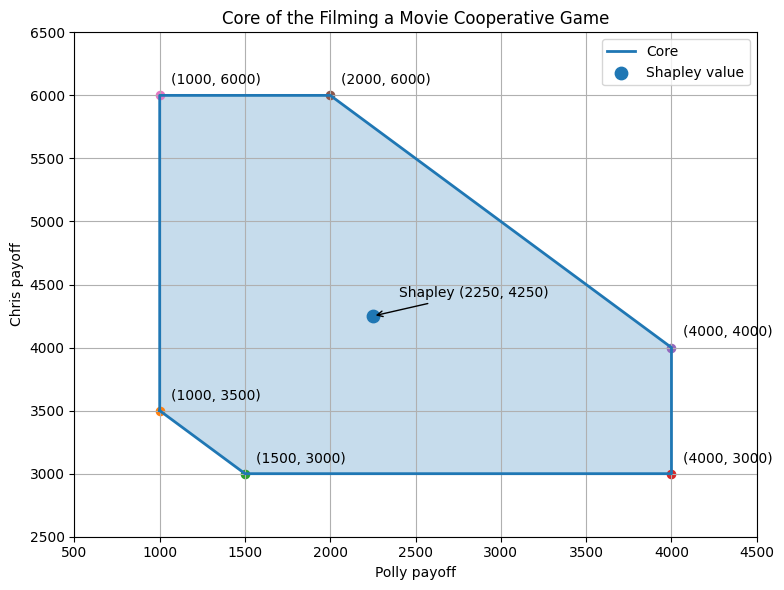
\includegraphics[width=1\textwidth]{problem3_1.png}
\end{center}

Now compute the Shapley value:

\[
\operatorname{sv}_P=\frac{1000+1000+2000+4000+1500+4000}{6}=2250,
\]
\[
\operatorname{sv}_O=\frac{3000+5500+2000+2000+5500+3000}{6}=3500,
\]
\[
\operatorname{sv}_C=\frac{6000+3500+6000+4000+3000+3000}{6}=4250
\]

\[
\begin{array}{c|ccc}
\text{Order} & P & O & C\\
\hline
POC & 1000 & 3000 & 6000\\
PCO & 1000 & 5500 & 3500\\
OPC & 2000 & 2000 & 6000\\
OCP & 4000 & 2000 & 4000\\
CPO & 1500 & 5500 & 3000\\
COP & 4000 & 3000 & 3000 \\
Shapley\ value & 2250 & 3500 & 4250
\end{array}
\]


Hence
\[
\operatorname{sv}(P,O,C)=(2250,3500,4250).
\]

Check whether it lies in the core:
\[
2250+3500+4250=10000,
\]
\[
2250\ge1000,\qquad 3500\ge2000,\qquad 4250\ge3000,
\]
\[
2250+3500=5750\ge4000,
\]
\[
2250+4250=6500\ge4500,
\]
\[
3500+4250=7750\ge6000
\]

Thus all core constraints are satisfied, so
\[
\operatorname{sv}(P,O,C)=(2250,3500,4250)\in \operatorname{Core}(v)
\]

Therefore,
\[
\text{the game is superadditive and supermodular,}
\]
and
\[
\text{the Shapley value lies inside the core}
\]

\vspace{1cm}

\end{document}
